\title{Analyzing Power Systems Stability \\ Using Contraction Theory}

\author{Liraz Nina Kalif \and Menashe Schwob} 
\date{\today}
\documentclass[12pt,English]{article}
\usepackage{graphicx}
\graphicspath{ {./images/} }
\usepackage{float}
\usepackage{preamble}

\begin{document}
\maketitle



\begin{abstract}
This is the paper's abstract \ldots
\end{abstract}
\newpage
\tableofcontents
\newpage
\listoffigures
\newpage
\section{Introduction}
\todo[inline]{some explanations about the importance of power systems and contraction theory}
\section{Background}
\subsection{Power Systems}
Power systems can be simple (one generator connected to an infinite bus), but can become more complex by adding components (more generators or buses). In this project we will discuss two simple power systems: the single generator and an infinite bus system and a two generators system.\\ 
The following assumptions will be used:
\begin{enumerate}
\item The network is lossless, therefore the impedance is given by $z = jx_{s} $.
\item No reactive losses.
\item All the loads are connected to a generator's junction.
\end{enumerate}
The dynamic of a power system is given by the \textbf{power flow Equations}:
\begin{align*}
P_{i}&=\sum_{n=1}^{N}\left|V_{i}\right|\left|V_{n}\right|\left|y_{i,n}\right|\cos\left(\delta_{n}-\delta_{i}+\theta_{i,n}\right)+P_{L,i}\\
Q_{i}&=\sum_{n=1}^{N}\left|V_{i}\right|\left|V_{n}\right|\left|y_{i,n}\right|\sin\left(\delta_{n}-\delta_{i}+\theta_{i,n}\right)+Q_{L,i}
\end{align*}
but can also be calculated directly.\\
A power system includes at least one generator that supplies the needed power. the generator is modeled by the \textbf{swing equation}:
\begin{align*}
\frac{d}{dt}\omega_{i}&=K\left(3P_{ref}-3P_{i}-\frac{1}{D}\left(\omega_{i}-\omega_{s}\right)\right)\\
\frac{d}{dt}\delta_{i}&=\omega_{i}-\omega_r   
\end{align*}
When:
\begin{itemize}
\item $P_ref$ is the power the generator is expected to supply (one phase).
\item $P_i$ is the power the generator is providing (one phase).
\item $D$ is the damping coefficient.
\item $\omega$ is the system's frequency.
\item $\omega_s$ is the work frequency of the system.
\item $\omega_r$ is the relative frequency for the generator.
\end{itemize}
\subsubsection{Stability of Power Systems}
When designing a power system, you must ensure that the system is \textbf{stable}, meaning that if the conditions change a little, the system will return to the stable state. \\
This is important because numerous components of the system depend on the stable state's features (such as the frequency) and can not endure large changes.  


\subsubsection{One Generator and Infinite Bus}

\begin{figure}[H]
\begin{center}
\includestandalone{\tikzfolter/infinity_bus_and_one_generator_one_line_diagram}
\end{center}
\caption{One Generator and Infinite Bus System}
\end{figure}


\begin{figure}[H]
\begin{center}
\includegraphics[]{\codefolter/unit_circles}
\end{center}
\caption{One Generator and Infinite Bus System}
\end{figure}

\begin{figure}[H]
\begin{center}
\includestandalone{\tikzfolter/infinity_bus_and_one_generator_circuit}
\end{center}
\caption{One Generator and Infinite Bus System}
\end{figure}

% \begin{figure}[H]
% \begin{center}
% 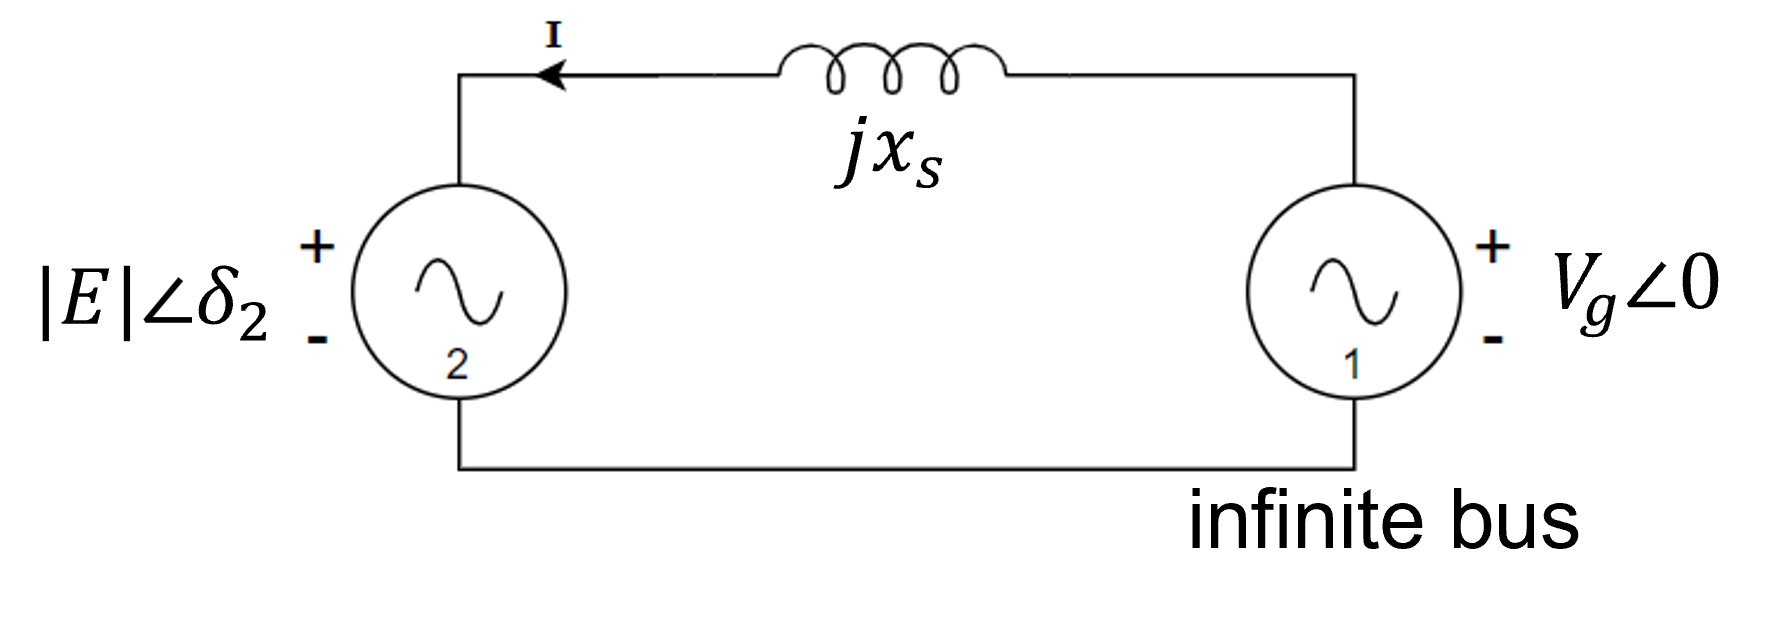
\includegraphics{one_gen.png}\\
% \end{center}
% \caption{One Generator and Infinite Bus circuit}
% \end{figure}

To analyse the system, the state-space equations are needed.\\
The current I:
\begin{align*}
I &= \frac{1}{Z}\left(\left|E\right|e^{j\delta_2}-V_g\right)\\
&= \frac{1}{jx_s}\left(\left|E\right|e^{j\delta_2}-V_g\right)
\end{align*}
The power supplied by the generator:
\begin{align*}
P &= \Re\left\{\left|E\right|e^{j\delta_2}I^*\right\}\\
&= \Re\left\{\left|E\right|e^{j\delta_2}\cdot\left(\frac{1}{-jx_s}\left(\left|E\right|e^{-j\delta_2}-V_g\right)\right)\right\}\\
&= \Re\left\{\frac{1}{-jx_s}\left[\left|E\right|^{2}e^{j\delta_2}e^{-j\delta_2}-\left|E\right|e^{j\delta_2}V_g\right]\right\}\\
&=  \Re\left\{\frac{j}{x_s}\left[\left|E\right|^{2}-\left|E\right|V_g\left(\cos{\delta_2}+j\sin{\delta_2}\right)\right]\right\}\\
&= \frac{\left|E\right|V_g\sin{\delta_2}}{X_s}\sin{\delta_2}=a_{21}\sin{\delta_2}
\end{align*}
And the state-space equations are:
\begin{align*}
\frac{d}{dt}\omega&=K\left(3P_{ref}-3\left(a_{21}\sin{\delta_2}\right)-\frac{1}{D}\left(\omega-\omega_{s}\right)\right)\\
\frac{d}{dt}\delta_2&=\omega-\omega_s   
\end{align*}
The Jacobian is given by:
\begin{align}\label{one_gen_J}
J=\left[\begin{array}{cc}
-\frac{K}{D} & -3Ka_{21}\cos{\delta_2}\\
1 & 0
\end{array}\right]    
\end{align}


\subsubsection{Two Generators}

\begin{figure}[H]
\begin{center}
\includestandalone{\tikzfolter/two_generators_one_line_diagram}
\end{center}
\caption{Two Generators System}
\end{figure}

\begin{figure}[H]
\begin{center}
\includestandalone{\tikzfolter/two_generators_circuit}
\end{center}
\caption{Two Generators System}
\end{figure}

% \begin{figure}[H]
% \begin{center}
% 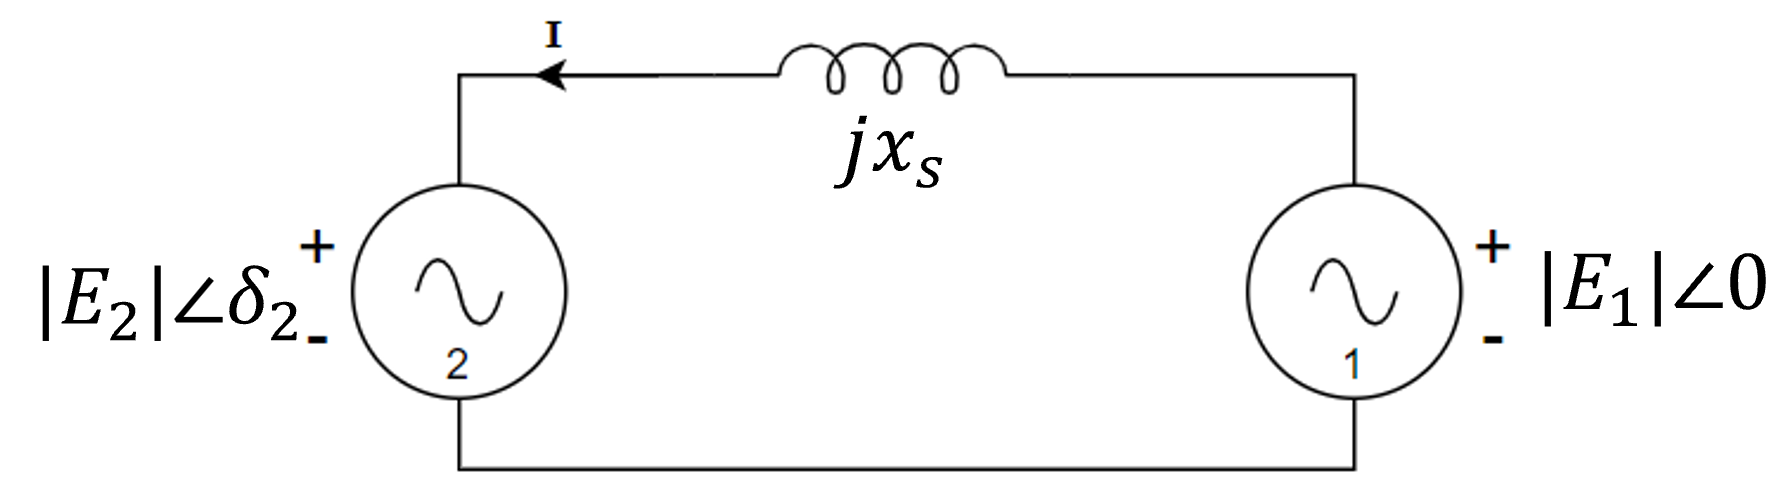
\includegraphics{two_gen.png}\\
% \end{center}
% \caption{Two Generators circuit}
% \end{figure}

To analyse the system, the state-space equations are needed.\\
The current I:
\begin{align*}
I &= \frac{1}{Z}\left(\left|E_2\right|e^{j\delta_2}-\left|E_1\right|\right)\\
&= \frac{1}{jx_s}\left(\left|E_2\right|e^{j\delta_2}-\left|E_1\right|\right)   
\end{align*}
The power supplied by generator 2:
\begin{align*}
P_2 &= \Re\left\{\left|E_2\right|e^{j\delta_2}I^*\right\}\\
&= \Re\left\{\left|E_2\right|e^{j\delta_2}\cdot\left( \frac{1}{-jx_s}\left(\left|E_2\right|e^{-j\delta_2}-\left|E_1\right|\right)\right)\right\}\\
&= \Re\left\{\frac{1}{-jx_s}\left[\left|E_2\right|^{2}e^{j\delta_2}e^{-j\delta_2}-\left|E_2\right|\left|E_1\right|e^{j\delta_2}\right]\right\}\\
&= \Re\left\{\frac{j}{x_s}\left[\left|E_2\right|^{2}-\left|E_2\right|\left|E_1\right|\left(\cos{\delta_2}+j\sin{\delta_2}\right)\right]\right\}\\
&= \frac{\left|E_2\right|\left|E_1\right|}{X_s}\sin{\delta_2}=a_{21}\sin{\delta_2}
\end{align*}
From power conservation:
\begin{align*}
    P_1 = -P_2 = -a_{21}\sin{\delta_2}
\end{align*}
And the state-space equations are:
\begin{align*}
\frac{d}{dt}\omega_1&=K_1\left(3P_{1,ref}+3\left(a_{21}\sin{\delta_2}\right)-\frac{1}{D_1}\left(\omega_1-\omega_{s}\right)\right)\\
\frac{d}{dt}\omega_2&=K_2\left(3P_{2,ref}-3\left(a_{21}\sin{\delta_2}\right)-\frac{1}{D_2}\left(\omega_2-\omega_{s}\right)\right)\\
\frac{d}{dt}\delta_2&=\omega_2-\omega_1   
\end{align*}
The Jacobian is given by:
\begin{align}\label{two_jen_J}
J=\left[\begin{array}{ccc}
-\frac{K_1}{D_1} & 0 & 3K_1a_{21}\cos{\delta_2}\\
0 & -\frac{K_2}{D_2} & -3K_2a_{21}\cos{\delta_2}\\
-1 & 1 & 0
\end{array}\right]    
\end{align}


\subsection{Methods to Find Stability Areas}
\subsubsection{linearization}
\todo[inline]{one paragraph about linearization, pros and cons}
\subsubsection{Lyapunov Criteria}
\todo[inline]{how much do we want/need to explain? pros and cons}
\subsubsection{Contraction Theory}

\subsection{Contraction Theory}
\todo[inline]{one paragraph about the motivation and the general idea. pros and cons}

\subsubsection{Vector Norms, Matrix Norms and Matrix Measures}
\paragraph{Vector Norms}\hfill\break
A vector norm defines a magnitude of vectors.
\begin{defn}
A vector norm $\left|\cdot\right|$ is a function $\left|\cdot\right|:\mathbb{R}^{n}\rightarrow\mathbb{R}^{+}$
such that for all $x,y\in\mathbb{R}^{n}$:
\begin{enumerate}
\item positive definiteness: $\left|x\right|\geq0$ and $\left|x\right|=0$
if and only if $x=0$.
\item absolute homogeneity: $\left|\alpha x\right|=\left|\alpha\right|\cdot\left|x\right|$
for any $\alpha\in\mathbb{R}$.
\item triangle inequality: $\left|x+y\right|\leq\left|x\right|+\left|y\right|$.
\end{enumerate}
\end{defn}
%
One of the most commonly used types of norms is $p$-norms, $L_{p}$.
\begin{defn}
Given a vector space $\mathbb{R}^{n}$, for any $p\in\mathbb{N}$
the vector norms $L_{p}$, denoted by $\left|\cdot\right|_{p}$ is
defined such that for all $x=\left(x_{1},\dots,x_{n}\right)\in\mathbb{R}^{n}$
$$
\left|x\right|_{p}\coloneqq\left(\sum_{k=1}^{n}\left|x_{k}\right|^{p}\right)^{\frac{1}{p}}
$$
for $p=\infty$, the $L_{\infty}$ vector norm is defined by
$$
\left|x\right|_{\infty}\coloneqq\max_{i\in\left\{ 1,\dots,n\right\}}\left|x_{i}\right|
$$
\end{defn}
%
In our work we will use the $L_{p}$ norms. In particular, we will use $L_{1},L_{2},L_{\infty}$.


\begin{figure}[h]
\begin{center}
\mbox{

\begin{subfigure}[t]{0.3\textwidth}
\centering
\includestandalone{\tikzfolter/L1_unit_circle}
\caption{$\left|x\right|_{1}=\sum\limits_{i=0}^{n}\left|x_{i}\right|$}
\end{subfigure}

\hspace{2em}
\begin{subfigure}[t]{0.3\textwidth}
\centering
\includestandalone{\tikzfolter/L2_unit_circle}
\caption{$\left|x\right|_{2}=\sqrt{\sum\limits_{i=0}^{n}\left|x_{i}\right|^{2}}$}
\end{subfigure}

\hspace{2em}
\begin{subfigure}[t]{0.3\textwidth}
\centering
\includestandalone{\tikzfolter/Linf_unit_circle}
\caption{$\left|x\right|_{\infty}=\max\limits_{i\in\left\{ 1,\dots,n\right\}}\left|x_{i}\right|$}
\end{subfigure}

}
\end{center}
\caption{The Unit circle for $L_{1},L_{2},L_{\infty}$ norms}
\end{figure}




\paragraph{Matrix Norms}\hfill\break
Norms can also be define on matrix (or equally, transformations). There are various types of matrix norms. In our work, we will only discuss so-called induced matrix norms\footnote{sometimes also called operator norms, or least upper bound norms.}.
\begin{defn}
Given a vector space $\mathbb{R}^{n}$ and a vector norm $\left|\cdot\right|$, the induced matrix norm $\left\Vert\cdot\right\Vert$ of an square\footnotemark{} matrix $A$ is a function $\left\Vert\cdot\right\Vert:\mathbb{R}^{n\times n}\rightarrow\mathbb{R}^{+}$ such that
\footnotetext{
The induced matrix norm can be more generally defined for rectangular
matrices, and with respect to two different vector norms: one measuring
the effect of applying the linear transformation $A$, and the other measuring
the size of the vector $x$ before the transformation. Such norms are in fact
also useful in some cases in contraction theory. However, we won’t need
them, so we will stick to square matrices and a single norm for $Ax$ and $x$.
}

$$
\left\Vert A\right\Vert \coloneqq\max_{x\in\mathbb{R}^{n}\backslash \left\{   0\right\}}\frac{\left|Ax\right|}{\left|x\right|}=\max_{\left|x\right|=1 , x\in\mathbb{R}^{n}}\left|Ax\right|
$$

\end{defn}
Since the matrix norm is induced by the vector norm, it satisfies similar properties. For all $A,B\in\mathbb{R}^{n\times n}$:
\begin{enumerate}
\item positive definiteness: $\left\Vert A\right\Vert\geq0$ and $\left\Vert A\right\Vert=0$
if and only if $A=0$.
\item absolute homogeneity: $\left\Vert\alpha A\right\Vert=\left|\alpha\right|\cdot\left\Vert A\right\Vert$
for any $\alpha\in\mathbb{R}$.
\item triangle inequality: $\left\Vert A+B\right\Vert\leq\left\Vert A\right\Vert+\left\Vert B\right\Vert$.
\item submultiplicativity: $\left\Vert AB \right\Vert\leq\left\Vert A\right\Vert\cdot\left\Vert B \right\Vert$.
\end{enumerate}

An additional useful property, which follows directly from the definition, is that
for any $A\in\mathbb{R}^{n\times n}$ and $x\in\mathbb{R}^{n}$ $$\left|Ax\right|\leq\left\Vert A \right\Vert\cdot\left|x\right|$$

A useful intuition for this induced matrix norm is that it measures the maximal expansion a linear transformation can cause when it is applied to any vector in the space. This is useful for our work since it give us a way to limit the maximum expansion of a vector in a system. This is very closely related to the linear discrete-time systems. For example, consider the system 
$$x\left(k+1\right)=Ax\left( k \right)t$$
then $\left\Vert A \right\Vert$ measures what is the maximal ratio which $\left|x\right|$ can grow between
time steps. If $\left\Vert A \right\Vert\leq1$, then $\lim_{k\rightarrow\infty}x\left(k\right)=0$. In fact, the matrix norm can be used to study contraction in discrete-time dynamical systems.

As mentioned above, in our work we will focus on $L_{1},L_{2},L_{\infty}$ norms, so in particular we will use the following matrix norms:
\begin{align}
&\left\Vert A\right\Vert_{L_1}=\max_{\left|x\right|=1 , x\in\mathbb{R}^{n}}\sum_{k=1}^{n}\left|x_{k}\right|
\\
&\left\Vert A\right\Vert_{L_2}=\max_{\left|x\right|=1 , x\in\mathbb{R}^{n}} \sqrt{\sum_{k=1}^{n}\left|x_{k}\right|^{2}}
\\
&\left\Vert A\right\Vert_{L_\infty}=\max_{\left|x\right|=1 , x\in\mathbb{R}^{n}} \max_{i\in\left\{ 1,\dots,n\right\}}\left|x_{i}\right|
\end{align}

\paragraph{Matrix Measures or logarithmic norms}\hfill\break
\begin{defn}
Given a vector space $\mathbb{R}^{n}$, a vector norm $\left|\cdot\right|$ and its induced matrix norm $\left\Vert\cdot\right\Vert$, the induced matrix measure of an square matrix $A$ defined by
$$\mu\left(A\right)\coloneqq\lim_{h\rightarrow0^+}\frac{\left\Vert I+hA\right\Vert-1}{h}$$
as $I$ is the identity matrix and $0<h\in\mathbb{R}$.
\end{defn}

This is essentially a directional derivative of the induced matrix norm in the
direction of A and evaluated at the identity matrix. In other words, the matrix measure gives information about the change of the matrix norms around the matrix $A$. For our definition of the matrix norm, the meaning is the change of the maximum expansion of vector cause by the linear transformation $A$.
\todo[inline]{rework on that explanation after understanding better the direction point}

For $L_{1},L_{2},L_{\infty}$ norms with the indueced matrix norm we defined above, it can be shown that the matrix measures for are given by\footnotemark
\begin{align}
&\mu_{L_1}\left(A\right)=\max_{j}\left\{ A_{jj}+\sum_{i=1,i\ne j}^{n}\left|A_{ij}\right|\right\}
\\
&\mu_{L_2}\left(A\right)=\lambda_{max}\left(\frac{A+A^{T}}{2}\right)
\\
&\mu_{L_\infty}\left(A\right)=\max_{i}\left\{ A_{ii}+\sum_{j=1,j\ne i}^{n}\left|A_{ij}\right|\right\}
\end{align}

\footnotetext{For simplicity, we will also use $\mu_1,\mu_2,\mu_\infty$ instead of $\mu_{L_1},\mu_{L_2},\mu_{L_\infty} $ }

\todo[inline]{
please add in your book a proof showing that for any $L_p$ norm, $\mu\left(A\right)\geq\max_i A_{ii}$, i.e. the matrix measure is bounded below by the diagonal entries of the matrix. As a hint, take the vector $e_1 = \left[1 0 \dots 0\right]^T$. What is $\left|e_1\right|$? What is the value of $Ae_1$? What is the relation between $\left|A_e1\right|$ and $\left\Vert A\right\Vert$
}

Matrix measures have plenty of interesting properties. Here are a few which
will be particularly interesting to us.

First,  a very powerful property of the matrix measure \todo[inline]{under which assumptions?} is that it invariant to \textit{similarity transformation}. Means, that applying an similarity transformation on a matrix does not change the matrix measure of it. This property allows to move the system to another coordinates system of another vector norm while preserving the matrix measure. It will be very useful since as it will be shown, it will be use to calculate the matrix measure associated with unknown $p$ norm using $L_{1},L_{2},L_{\infty}$ norms.
The following theorem and lemma will help on understanding this important point.

\begin{thm}
Let $T\in\mathbb{R}^{n\times n}$ an invertible matrix.
Given a vector space $\mathbb{R}^{n}$ and a vector norm $\left|\cdot\right|$, for all $x\in\mathbb{R}^{n}$,  the function denoted by $\left|\cdot\right|_{t}$ (t-norm)
\begin{equation}
    \left|x\right|_{t}\triangleq\left|Tx\right|
\end{equation}
is a vector norm.
\end{thm}

\begin{proof}\hfill
\begin{enumerate}
        \item positive definiteness: Let $x,y\in\mathbb{R}^{n}$ such that $y=Tx$, then $$\left|x\right|_{t}\triangleq\left|Tx\right|=\left|y\right|\geq0$$
        since $T$ is invertible, $T\ne0$ and
        $$x=0 \Rightarrow \left|x\right|_{q}=\left|Tx\right|=0$$
        $$\left|x\right|_{q}=0 \Rightarrow \left|Tx\right|=0 \Rightarrow x=0$$ 
        
        \item absolute homogeneity: for any $\alpha\in\mathbb{R}$, 
        $$\left|\alpha x\right|_{t}=\left|T\left(\alpha x\right)\right| =\alpha\left|Tx\right|=\alpha\left|x\right|_{t}$$
        
        \item triangle inequality: for any $x,y\in\mathbb{R}^{n}$,
        $$\left|x+y\right|_{t}=\left|T\left(x+y\right)\right|=\left|Tx+Ty\right|\leq\left|Tx\right|+\left|Ty\right|=\left|x\right|_{t}+\left|y\right|_{t}$$

    \end{enumerate}
\end{proof}


\begin{lem}
Let $T\in\mathbb{R}^{n\times n}$ an invertible matrix.
Given a vector space $\mathbb{R}^{n}$ and a vector norm $\left|\cdot\right|$, the t-norm, $\left|\cdot\right|_{t}$, implement the following properties:
\begin{enumerate}
    \item $\left\Vert A\right\Vert _{t}=\left\Vert TAT^{-1}\right\Vert$
    \item $\mu_{q}\left(A\right)=\mu\left(TAT^{-1}\right)$
\end{enumerate}
\end{lem}

\begin{proof}\hfill
\begin{enumerate}
    \item Consider $x\in\mathbb{R}^{n}$ such that $v=Q^{-1}x$, then
        \begin{align*}
            \left\Vert A\right\Vert _{t} & =\underset{v\in\mathbb{R}^{n}}{\max}\frac{\left|Av\right|_{t}}{\left|v\right|_{t}}
            =\underset{v\in\mathbb{R}^{n}}{\max}\frac{\left|TAv\right|}{\left|Tv\right|}\\
            &=\underset{x\in\mathbb{R}^{n}}{\max}\frac{\left|TAT^{-1}x\right|}{\left|TT^{-1}x\right|}
            =\underset{x\in\mathbb{R}^{n}}{\max}\frac{\left|TAT^{-1}x\right|}{\left|x\right|}
            =\left\Vert TAT^{-1}\right\Vert 
    \end{align*}
    \item 
    \begin{align*}
        \mu_{t}\left(A\right) & =\lim_{h\rightarrow0^{+}}\frac{\left\Vert I+hA\right\Vert _{t}-1}{h}\\
         & =\lim_{h\rightarrow0^{+}}\frac{\left\Vert T\left(I+hA\right)T^{-1}\right\Vert -1}{h}\\
         & =\lim_{h\rightarrow0^{+}}\frac{\left\Vert TIT^{-1}+hTAT^{-1}\right\Vert -1}{h}\\
         & =\lim_{h\rightarrow0^{+}}\frac{\left\Vert I+hTAT^{-1}\right\Vert -1}{h}\\
         & =\mu\left(TAT^{-1}\right)
\end{align*}
\end{enumerate}
\end{proof}

So as shown, given a system represented by matrix a $A$ and vector norm, any inverse transformation $T$ will define an another new norm which preserve the system matrix norm and matrix measure of the system under transformation. So the new matrix measure of the system can be calculated by the given matrix measure. 

\todo[inline]{explain that the transformation transform the p norm to another norm (not neccerly p norm) where the circle became ellipse} 


The next properties of the matrix measure gives an indication about the system stability.
\begin{lem}
Let $A\in\mathbb{R}^{n\times n}$. Then for any eigenvalue $\lambda\in\mathbb{C}$ of $A$
\begin{equation}
    \Re\left(\lambda\right)\leq\mu\left(A\right)
\end{equation}
\end{lem}

\todo[inline]{explanation}

\begin{lem}
Let $A\in\mathbb{R}^{n\times n}$. There exists a vector norm and an induced matrix measure such that $\mu\left(A\right)<0$ if and only if $A$ is stable. 
\end{lem}

\todo[inline]{explanation}


Finally, the matrix measure has the property of exponentially bounding the vector norm of any solution of a LTV system. This property will be much help later for the contraction theory.
\begin{lem}(Coppel's inequality)\label{Coppel's inequality}.
Consider the linear time varying system
\begin{equation}
    \Dot{x}\left(t\right)=A\left(t\right)x\left(t\right)
\end{equation}
Then for any solution of the system, we have that
\begin{equation}\label{LTV system}
    \left|x\left(t\right)\right|\leq\exp{\left(\int_0^t\mu\left(A\left(s\right)\right)ds\right)\left|x\left(0\right)\right|}
\end{equation}
for all $t\geq0$.
\end{lem}

\begin{proof}
\todo[inline]{ understand}
Let $x\left(t\right)$ denote some solution of \ref{LTV system}. Then,
\begin{align*}
    \left|x\left(t+\varepsilon\right)\right|- \left|x\left(t\right)\right|&= \left|x\left(t\right)+\varepsilon A\left(t\right)x\left(t\right)\right|- \left|o\left(\varepsilon\right)\right|
    \\&= \left|\left(I+\varepsilon A\left(t\right)\right)x\left(t\right)\right|- \left|x\left(t\right)\right|+ o\left(\varepsilon\right)
    \\&\leq  \left(\left\Vert I+\varepsilon A\left(t\right)\right\Vert-1\right) \left|x\left(t\right)\right|+o\left(\varepsilon\right)
\end{align*}

Dividing by $\varepsilon$ and taking the limit of $\varepsilon\rightarrow0^{+}$
yields that
\[
\frac{d}{dt}\left|x\left(t\right)\right|\leq\mu\left(A\left(t\right)\right)\left|x\left(t\right)\right|
\]
Using a comparision theorem (in particular Gr¨onwall’s inequality) gives that $\left|x\left(t\right)\right|$ is bounded above by the solution of the first-order linear differential equation $\dot{z}\left(t\right)=\mu\left(A\left(t\right)\right)z\left(t\right)$. For the initial condition $z\left(0\right)\left|x\left(0\right)\right|$, the solution of the first-order equation is $z\left(t\right)=\exp\left(\int_{0}^{t}\mu\left(A\left(t\right)\right)ds\right)z\left(0\right)$, and this completes the proof.

\todo[inline]{This proof is not entirely rigorous, but it can be made accurate using a couple more definitions. However, I don’t think this really helps understanding the result. I will also note that Gr\"{o}nwall’s inequality is also not difficult to prove, but I again don’t think it adds any intuition.}

\end{proof}


\subsubsection{Contraction Theory}
\todo[inline]{explanation about using the liaponov eq. here.}

\subsubsection{Finding Stability Areas using Contraction Theory}
The mathematical background from lat section gives the base required to get to the main point, the contraction theory.

Consider the dynamic system
\begin{equation}\label{dynamical system}
    \dot{x}=f\left(t,x\right)
\end{equation}

with $x\in\Omega\subseteq\mathbb{R}^{n}$ and $\Omega$ is convex
and invariant set of dynamics \footnote{A set is called an invariant set of the dynamics, if every initial condition in the set yields a solution which remains in the set for all times}. For simplicity the initial time will be set to $0$. Let $J\left(t,x\right)$ denote the Jacobian of $f\left(t,x\right)$ with respect to $x.$ Let $x\left(t,a\right)$ denote the solution to \ref{dynamical system} with $x\left(0\right)=a$. 

On such system, \ref{dynamical system}, the system is a contraction in $\Omega$ if the distance between any two solution decays at an exponential rate.
\begin{defn}
Given a vector norm $\left|\cdot\right|$, a dynamical system $\dot{x}=f\left(t,x\right)$ with $x\in\Omega\subseteq\mathbb{R}^{n}$ and $\Omega$ is convex and invariant set is contraction with respect to $\left|\cdot\right|$ and rate $\eta>0$ if 
\begin{equation}\label{contraction definition}
    \left|x\left(t,a\right)-x\left(t,b\right)\right|\leq\left|a-b\right|e^{-\eta t}
\end{equation}

for any $a,b\in\mathbb{R}^{n}$ and $t\geq0.$
\end{defn}
%
\begin{thm}
Let $\left|\cdot\right|$denote some vector norm and $\mu\left(\cdot\right)$ denote the induced matrix measure. If
\[
\mu\left(J\left(t,x\right)\right)\leq-\eta<0
\]
for all $t\geq0$ and $x\in\Omega$, then \ref{dynamical system} is contraction with respect to norm $\left|\cdot\right|$ and rate $\eta$.
\end{thm}
\begin{proof}
Let $a,b\in\Omega.$ Define $w\left(t,r\right)\coloneqq\frac{\partial}{\partial r}x\left(t,ra+\left(1-r\right)b\right).$ Then, 
\begin{align*}
\frac{d}{dt}w\left(t,r\right) & =\frac{d}{dt}\frac{\partial}{\partial r}x\left(t,ra+\left(1-r\right)b\right)\\
 & =\frac{\partial}{\partial r}\frac{d}{dt}x\left(t,ra+\left(1-r\right)b\right)\\
 & =\frac{\partial}{\partial r}f\left(t,ra+\left(1-r\right)b\right)\\
 & =J\left(t,ra+\left(1-r\right)b\right)w\left(t,r\right)
\end{align*}
The LTV system $\dot{w}\left(t,r\right)=J\left(t,ra+\left(1-r\right)b\right)w\left(t,r\right)$ is the somethings called the \textit{variational equation} associated with \ref{dynamical system} along the solution $x\left(t,ra+\left(1-r\right)b\right).$ Intuitively, it described how small changes in the initial condition along the line connecting $a$ and $b$ evolves and effects the solution at time $t$. 

By the triangle inequality 
\begin{align*}
\left|\int_{0}^{1}w\left(t,r\right)dr\right| & \leq\int_{0}^{1}\left|w\left(t,r\right)\right|dr\\
 & \leq\int_{0}^{1}e^{-\eta t}\left|w\left(0,r\right)\right|dr\\
 & =e^{-\eta t}\int_{0}^{1}\left|a-b\right|dr\\
 & =e^{-\eta t}\left|a-b\right|
\end{align*}
where we used Coppel's inequality \todo[inline]{add steps and why linear is ok here} \ref{Coppel's inequality} in the second inequality. Using the Fundamental Theorem of Calculus, we have that
\[
\left|\int_{0}^{1}w\left(t,r\right)dr\right|=\left|x\left(t,a\right)-x\left(t,b\right)\right|
\]
and this completes the proof.
\end{proof}


\section{Numerical Experiments}
the experiments that didn't work % TODO if we want to include them
\section{One Generator and Infinite Bus Simulation}
\ref{one_gen_J} need to find a way to include graphs
\section{Two Generators Simulation}
\section{Open Questions and Ongoing Research}
open questions here
\section{Conclusion}
The conclusion goes here.
\section*{Acknowledgment}
The authors would like to thank...
\section*{bibliography}

\end{document}
